\chapter{Présentation des frameworks d'édition d'images (15 pages) }
	
	Dans ce mémoire nous discuterons d'un ensemble d'algorithmes constituant un framework
	de rendu et d'édition d'images nommé \emph{Himalaya}. Par le terme framework nous entendons une
	librairie présentant une interface logicielle permettant a un utilisateur d'éditer des images. \index{Framework d'edition d'images}
	Par utilisateur nous entendons l'artiste qui utilise un logiciel d'éditon, le programmeur qui utilise le framework pour
	concevoir un logiciel, mais aussi un autre programme qui ferait appel à celui ci.  De tels frameworks sont en effet utilisés
	par des applications fort variées, comme les logiciels de peinture, d'édition 3D, les jeux vidéos, les logiciels de cartographie,
	les interfaces multimédias, etc.

	Nous allons tout d'abord examiner quels sont les éléments qui consitituent un tel framework, ensuite quels sont
	les fonctionalités qu'ils doivent présenter à l'utilisateur et enfin les différentes manières de les implémenter,
	afin de voir où se situe \emph{Himalaya} dans le paysage des frameworks d'édition d'images.

	Pour réaliser cette présentation je me suis basé sur une lecture du code source des différents frameworks open-source, afin d'évaluer
	les structures de données et les algorithmes utilisés. Je me suis ausi basé sur les fonctionalités et leurs performances dans des
	logiciels fermés. Enfin, une étude des spécifications des principaux formats de fichiers standards permet de se rendre compte des
	fonctionalités qui sont attendues dans les frameworks. 

	

	\section{Architecture d'un framework d'édition d'image}
		Un framework d'édition d'images est composé de trois éléments principaux : 
		\begin{description}
			\item[Schéma de représentation de l'image]: Ce schéma est consititué de structures de données qui 
			décrivent l'image et les modifications qui lui sont apportées. 
			\item[Algorithme de rasterisation]: Cet algorithme permet d'obtenir une version matricielle de l'image,
			ou d'une partie de celle-ci. Une telle opération est indispensable car seule la forme matricielle de l'image
			peut être affichée ou imprimée. 
			\item[Algorithmes d'édition du schéma]: Ces algorithmes vont modifier la représentation de l'image afin 
			d'implémenter les différentes fonctionalités du framework.
		\end{description}

	\section{Fonctionalités d'un framework d'édition d'image}
		\subsection{Opérations de dessin}
			L'opération de base d'un framework d'édition d'image est bien évidemment de permettre de 
			modifier une image. On distingue plusieurs manières de le faire qui seront traitées différemment
			selon les implémentations.
			\subsubsection{Dessin de primitives}
				Par dessin de primitive on entend l'ajout sur l'image de primitives géométriques, comme
				des polygones, des lignes, des points, des ellipses, du texte, etc. Ces primitives ont généralement un 
				effet local sur l'image, c'est à dire qu'elles ne la modifient pas dans son intégralité. On s'attend généralement
				de la part d'un framework d'édition d'image que de telles opérations soient peu couteuse en
				temps et en mémoire, étant donné que la réalisation d'un dessin intéressant nécessite généralement
				un nombre très élevé de primitives, qui peut se compter en millions.
				\index{Primitives, dessin de}
				\begin{figure}[h]
					\centering
					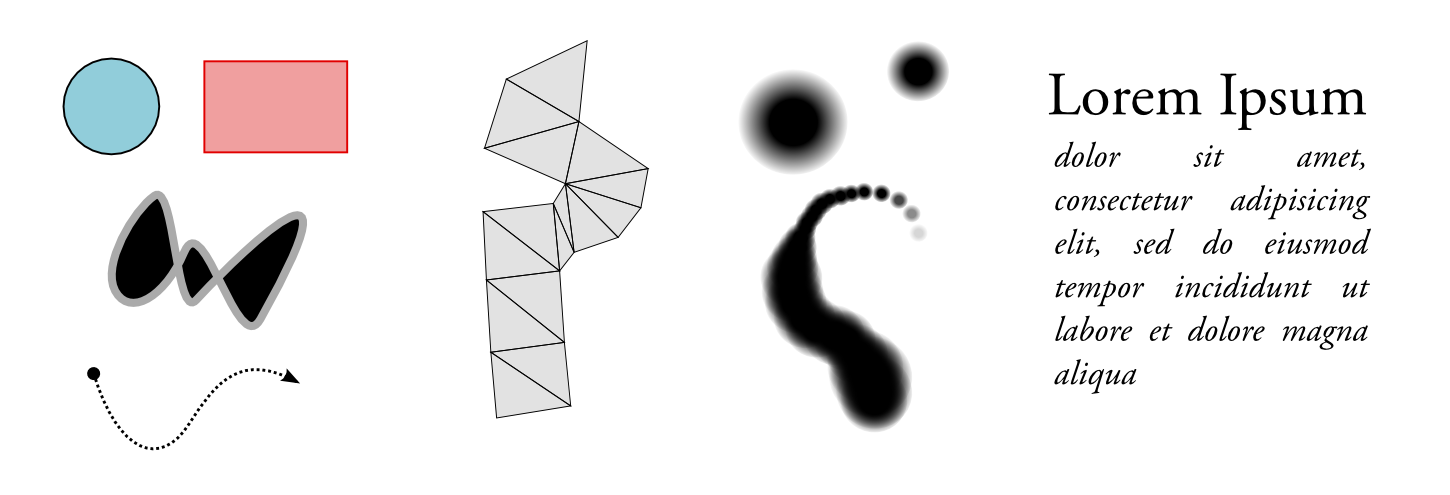
\includegraphics[width=\textwidth]{images/primitives}
					\caption{Examples de dessins de primitives}
					\label{fig:primitives}
				\end{figure}
			\subsubsection{Filtres}
				\index{Filtres}
				Un filtre est une opération qui modifie l'aspect de l'entièreté d'une image. Le temps de calcul d'un filtre varie
				énormément d'un filtre à l'autre. Les plus simples prennent quelques microsecondes et peuvent aisément être exécutés
				en temps réel. D'autres prennent plusieurs dixaines de minutes. Certains frameworks ne sauront intégrer que les filtres
				les plus rapides. 

				Les filtres peuvent être également partagés en deux catégories,\index{Filtres!colorimetriques} les filtres colorimétriques qui transforment
				la couleur d'un pixel sans se soucier de la couleur des pixels voisins, \index{Filtres!spatiaux} et les filtres spatiaux nécessitant 
				eux d'en connaître plusieurs. 
				\begin{figure}[h]
					\centering
					\subfloat[Image originale]{ \label{fig:lenna} 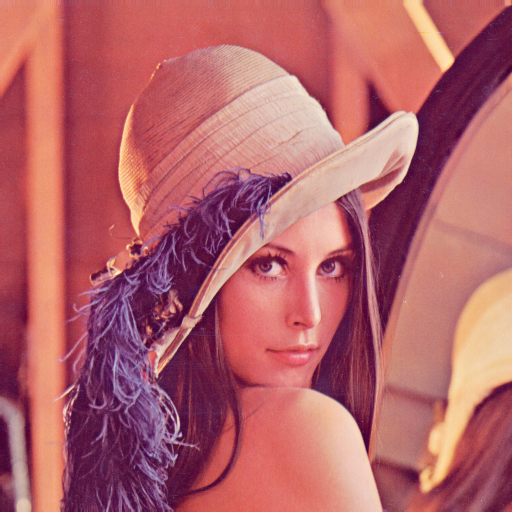
\includegraphics[width=0.3\textwidth]{images/Lenna} }
					\subfloat[Filtre colorimétrique]{ \label{fig:lenna} 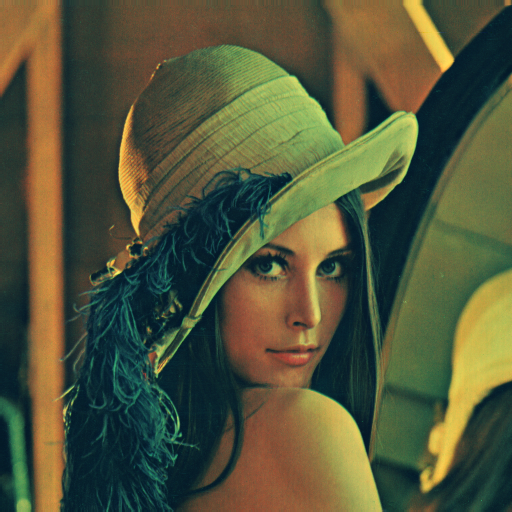
\includegraphics[width=0.3\textwidth]{images/Lenna-green} }
					\subfloat[Filtre spatial \emph{Sobel}]{ \label{fig:lenna} 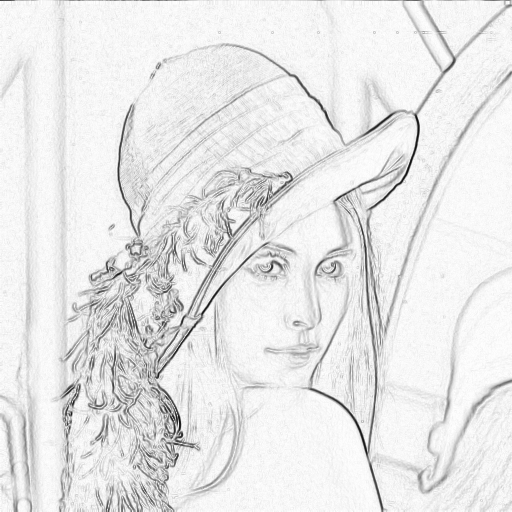
\includegraphics[width=0.3\textwidth]{images/Lenna-sobel} }
					\caption{Examples de filtres}
					\label{fig:filtres}
				\end{figure}
			\subsubsection{Transformations géométriques}
				Les transformations géométriques modifient la forme d'un objet constituant l'image; rotation, translation, 
				redimentionnement et perspective sont les applications les plus courantes. 
				
			\subsubsection{Fusion et modes de fusion}
				La fusion consiste à fusionner deux images de même taille en les superposant via une fonction spécifique s'appliquant pixel par pixel.
				Cette fonction est nommée \emph{mode de fusion} et a la forme $f(p_A ,p_B ,\alpha)$, où $p_A$, $p_B$ sont deux pixels 
				de coordonnées identiques appartenant aux deux images à fusionner. $\alpha$ représente un ou plusieurs paramètres additionnels qui peuvent
				modifier l'effet de la fonction.

				Le \emph{mode de fusion} la plus courante est celui de mélange par opacité: $f(p_A, p_B, \alpha) = \alpha * p_A + (1-\alpha) * p_B$,  $\alpha \in [0,1]$ 
				représentant l'opacité de $B$.

				Puisque chaque dessin de primitive consiste en la fusion de celle ci sur l'image de fond, la fusion est une opération centrale
				dans tout framework. Cependant beaucoup d'entre eux se limitent au seul mode de mélange par opacité.

				\begin{figure}[h]
					\centering
					\subfloat[Image A]{ \label{fig:A} 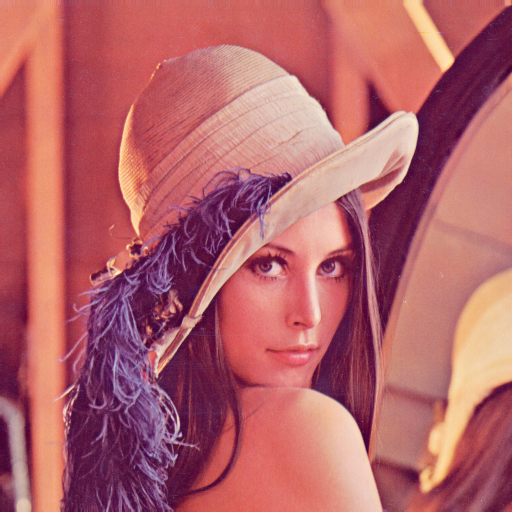
\includegraphics[width=0.25\textwidth]{images/Lenna} }
					\subfloat[Image B]{ \label{fig:B} 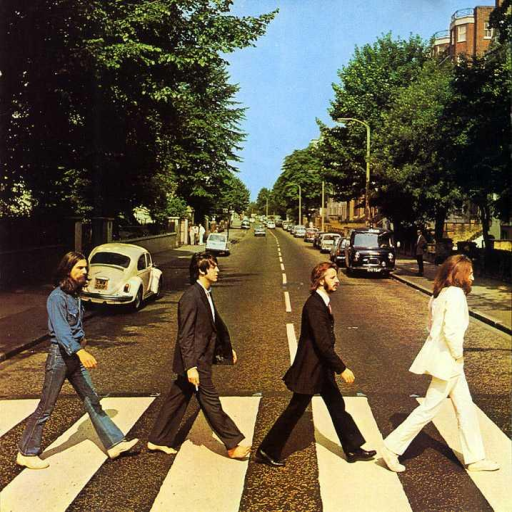
\includegraphics[width=0.25\textwidth]{images/abbey-road} }
					\subfloat[Blending de B sur A, par \emph{fusion de grain} ]{ \label{fig:ABfusion} 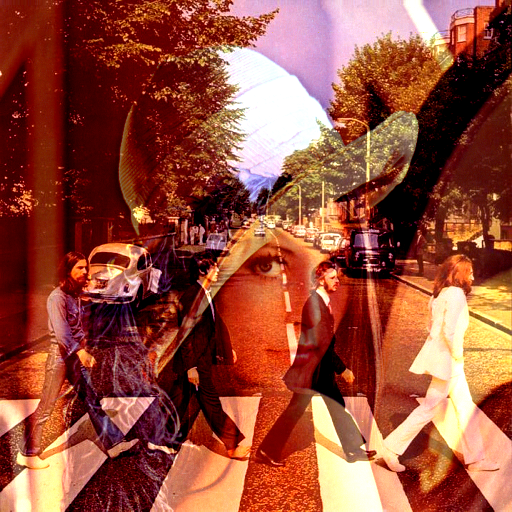
\includegraphics [width=0.25\textwidth]{images/abbey-road-lenna-fusion} }
					\subfloat[Blending de B sur A, par \emph{soustraction} ]{ \label{fig:ABsoustraction} 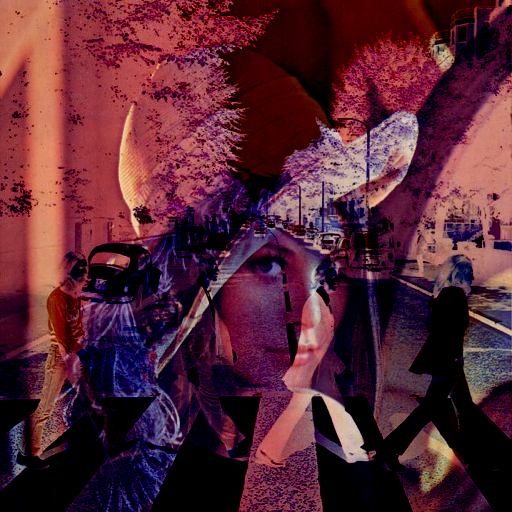
\includegraphics [width=0.25\textwidth]{images/abbey-road-lenna-substract} }
					\caption{Examples de blending}
					\label{fig:blending}
				\end{figure}

		\subsection{Modèles colorimétriques}
			La rasterisation d'une image permet de définir la couleur de chaque pixel. Or il existe de nombreuses manières de définir une même couleur.
			La manière la plus populaire est de définir la couleur comme un vecteur dans un espace colorimétrique. Chaque espace ayant sa propre utilité:
			\begin{description}
				\item[Le RGB] est l'espace utilisé par les écrans et projecteurs, ainsi que les capteur photographiques. Toute couleur doit donc être
				convertie en RGB avant d'être affichée. Il existe plusieurs espaces RGB définis par des couleurs primaires Rouges, Vertes et Bleues différentes.
				Le plus utilisé est le sRGB, qui est le standard d'affichage des écrans.
				\item[Le Yuv] est l'espace utilisé par les vidéos et par certains formats de fichier comme le JPEG.
				L'espace Yuv permet en effet une meilleure compression des données.
				\item[Le CIELab] est l'espace utilisé en retouche photo, il permet de manipuler les couleurs de manière conforme à la perception humaine.
				\item[Le HSL] est un espace qui permet de décrire les couleurs en composantes de teintes, de saturation et de luminosité, notions
				facilement compréhensibles et manipulables. Cet espace est utilisé pour certains filtres et pour l'édition des couleurs.
				\item[Le CMYK] est l'espace utilisé par les imprimantes jet d'encre, chaque imprimante ayant ses propres couleurs primaires. 
				Toute image doit donc être convertie dans le CMYK correspondant à l'imprimante avant d'être imprimée.
			\end{description}
			Il existe encore bien d'autres espaces colorimétriques spécifiques à des applications industrielles particulières. 

			Pour compliquer le tout, les espaces colorimétriques ne se supperposent généralement pas. Ainsi des couleurs qui peuvent s'exprimer dans l'un n'existent pas
			dans l'autre. Un framework dédié à l'impression doit ainsi prendre garde de n'afficher en RGB que des couleurs disponibles dans le CMYK de l'imprimante.

			Une autre manière de décrire les couleurs est d'utiliser une palette de couleurs standard. Ce système est utilisé dans les images destinées à l'impression
			afin d'identifier des encres dont l'apparence ne peut être réduite à une simple couleur, comme les encres mattes, brillantes, métallisées,
			fluorescentes, etc. Dans ce cas chaque pixel possède une certaine quantité de chacune des  couleurs utilisées pour décrire l'image.

			\subsubsection{Quantisation}
			Les composantes d'un pixel peuvent aussi être quantifiées à différents degrés: 1bit pour les systèmes halftone; 8bit pour l'affichage 
			à l'écran,  les textures de jeux vidéos; 32 bit flottant permet d'avoir des valeurs de couleurs dépassant les capacité d'affichage
			d'un écran, ce qui est particulièrement intéressant pour l'édition non destructive d'image utilisée en photographie et en 
			effets spéciaux. La précision apportée par une telle profondeur est également indispensable pour le cinéma numérique.

			\subsubsection{Au delà de la couleur}

			Enfin, il arrive qu'un pixel ne décrive plus une couleur mais une information quelconque de lá partie de l'objet qu'il représente.
			On rencontre ainsi la distance du pixel à l'observateur, la normale de la surface, un identifiant unique de l'objet, la vitesse de
			déplacement de l'objet, etc.

			Ce type d'information est typiquement fourni par la caméra ou généré par le moteur de rendu afin de faciliter l'intégration d'effets
			spéciaux à l'image. Le type d'information utilisés apparaissent et disparaissent avec les technologies, nécessitant une grande 
			flexibilité dans leur gestion. Les \emph{Éditeurs Nodaux} sont particulièrement adaptés à la gestion de ce type d'informations.
			
			\begin{figure}[h]
				\centering
				\subfloat[Couleurs vraies]{ \label{fig:render} 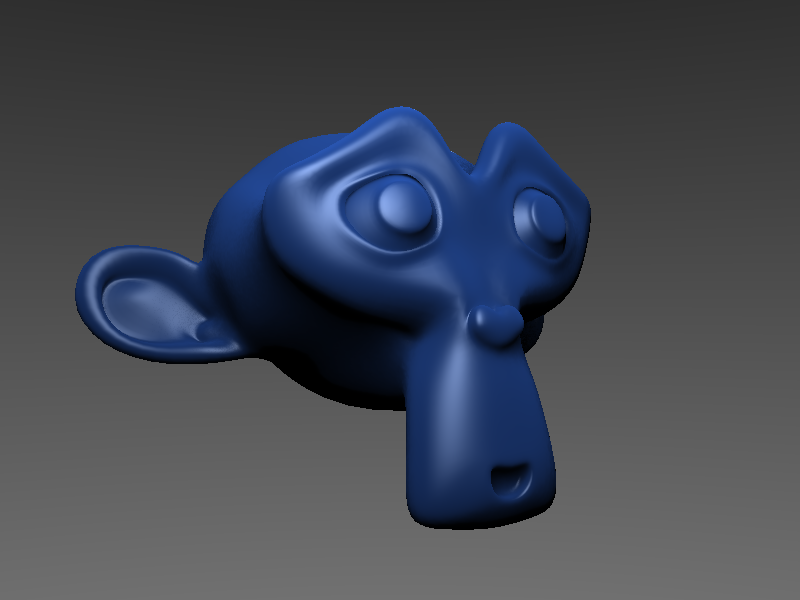
\includegraphics[width=0.25\textwidth]{images/render} }
				\subfloat[Format HSV en fausses couleurs]{ \label{fig:render-hsv} 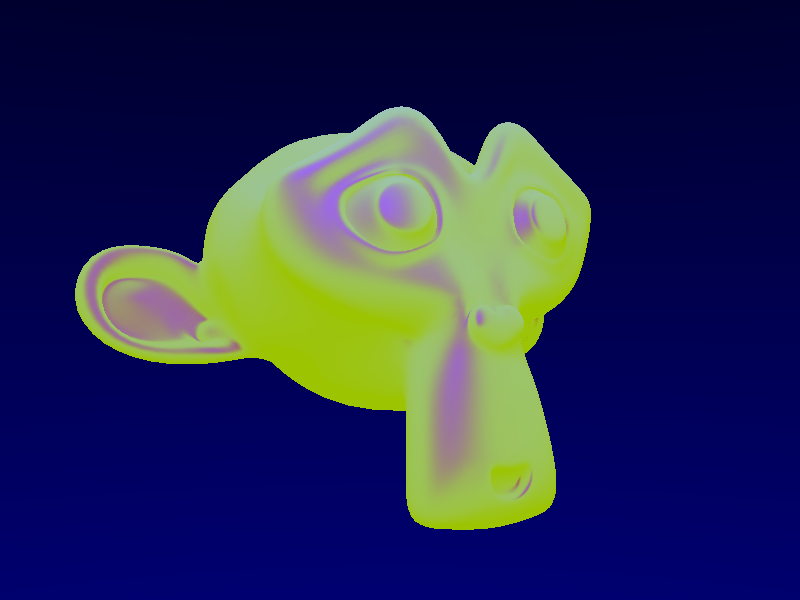
\includegraphics[width=0.25\textwidth]{images/render-hsv} }
				\subfloat[Vecteur normal de la surface]{ \label{fig:render-normal} 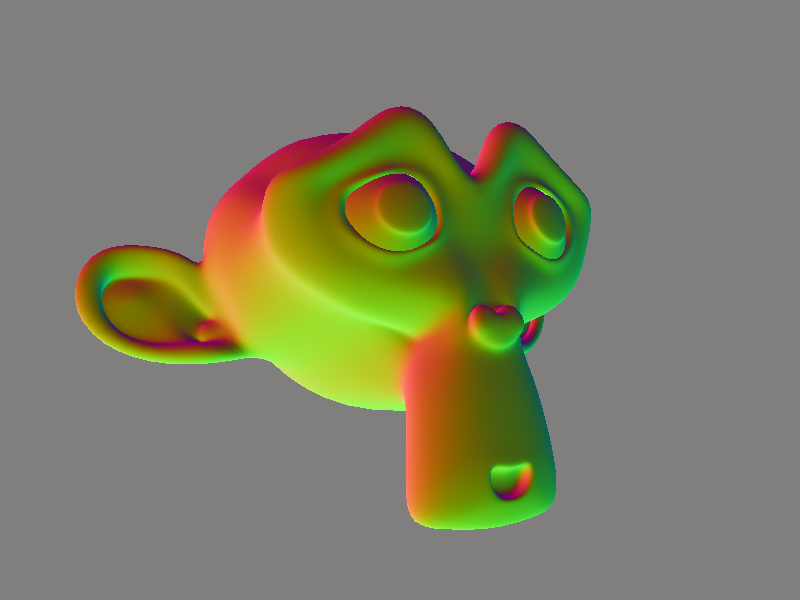
\includegraphics [width=0.25\textwidth]{images/render-normal} }
				\subfloat[Distance à l'observateur]{ \label{fig:render-depth} 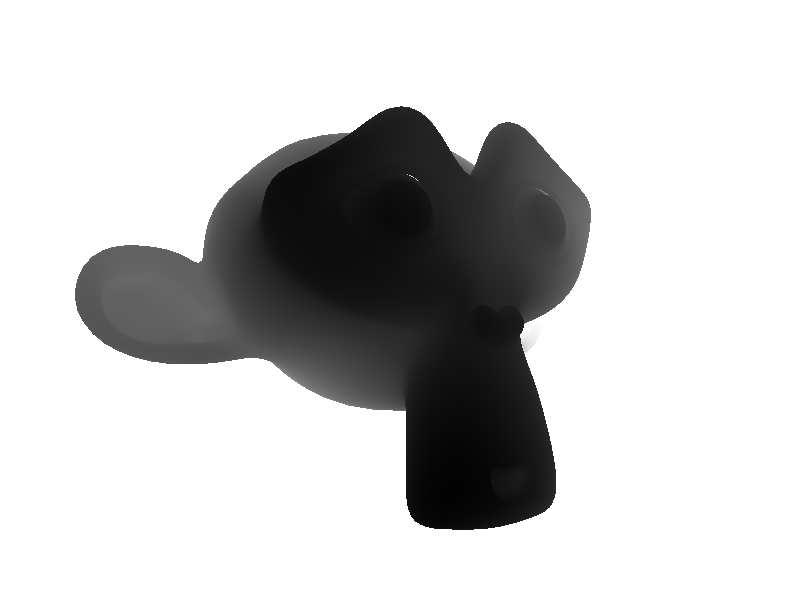
\includegraphics [width=0.25\textwidth]{images/render-depth} }
				\caption{Examples d'espaces colorimétriques et de métadonnées}
				\label{fig:color}
			\end{figure}

		\subsection{Undo / Redo}
			Un framework a souvent des mécanismes internes permettant une gestion efficace d'annulation et de répétiton des opérations.
		\subsection{Édition non destructive}
			L'édition non destructive consiste à pouvoir modifier les opérations après leur application sans perte de qualité de l'image.
		\subsection{Composition non linéaire}
			La composition non linéaire permet à une opération d'utiliser le résultat d'une opération que celle appliquée précedemment. Cette
			fonctionalité permet d'obtenir des effets complexes à partir d'opérations simples. 
		\subsection{Édition par pixel}
			Certains frameworks permettent d'éditer l'image au niveau des pixels individuels.
		\subsection{Indépendance de la résolution}
			Dans ce cas la description de l'image est indépendante de la résolution utilisée pour la rasterisation; Il n'y a pas de dégradation
			de la qualité de l'image quelque soit la résolution utilisée pour le rendu.
		\subsection{Images gigapixels}
			Les images gigapixels sont les images constituées de plus d'un milliard de pixel, qui sont généralement plus grandes que la mémoire
			vive disponible. Ces images sont utilisées de plus en plus fréquement et certains frameworks, dont \emph{Himalaya} sont particulièrement
			adaptés à la gestion de ce type d'images. 
		\subsection{Traitement d'images multiples}
			Le traitement d'images multiples consiste en savoir appliquer facilement les mêmes opérations sur un large nombre d'images similaires, 
			comme par exemple les photos d'une séance de shooting, les frames d'une vidéo ou d'un moteur 3D, si possible en temps réel.

	\section{Frameworks Bitmaps}

		\subsection{Schéma de représentation de l'image}
			\begin{figure}[h]
				\centering
				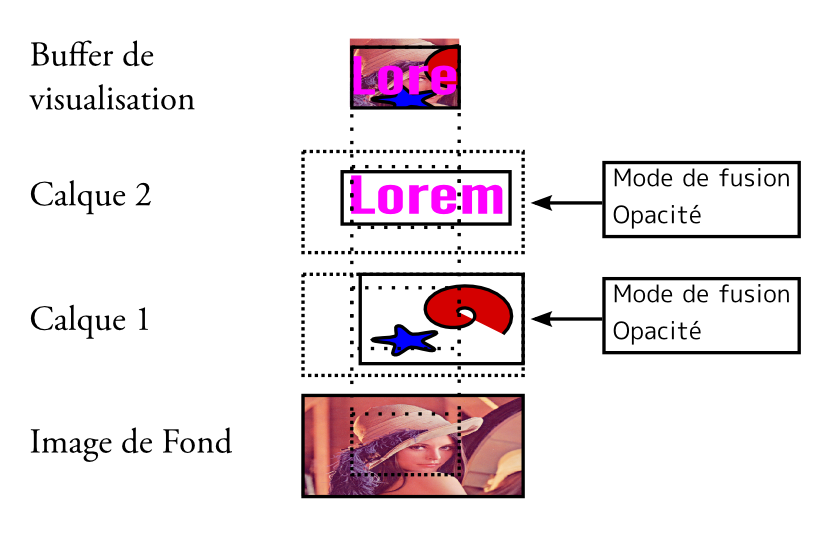
\includegraphics[width=0.6\textwidth]{images/calques}
				\caption{Représentation d'une image par calques}
				\label{fig:editbitmap}
			\end{figure}
			Dans un framework bitmap l'image est représentée directement sous sa forme rasterisée. 
			
			Une extension populaire est de décomposer l'image en une image de fond et une superposition de calques qui sont des bitmaps possèdant chacun leur propre
			dimension, position, un mode de fusion, et des paramètres d'opacité. Cette extension permet à l'utilisateur de pouvoir facilement modifier des zones
			spécifiques de l'image.

			Des frameworks extendent encore ce principent en décomposant les calques en sous calques, et ce de manière récursive. 

		\subsection{Algorithme de rasterisation}
			Dans un framework bitmap, chaque opération est directement rasterisée à la résolution native lors de son application. 
			
			Pour visualiser une région à une échelle différente de la résolution native, On utilise un buffer de visualisation de la taille
			de cette région dans lequel la région d'intérèt est mis à l'échelle voulue après chaque rasterisation.
			
			Lorsqu'un système de calques est utilisé, on rasterise d'abord directement l'opération sur le calque modifié. On place ensuite l'image
			de fond dans le buffer de visualisation. Chaque calque y est ensuite fusionné.			
			
			Comme la plupart des opérations ne modifie qu'une petite partie de l'image, on aimerait éviter de devoir fusionner l'intégralité
			des calques à chaque fois. Il y a deux approches pour cela: La première est de demander à chaque opération de spécifier la région
			qu'elle modifie. On ne modifie ensuite le buffer de visualisation que pour cette région. 

			La deuxième approche consiste à diviser l'image de fond et les calques en une grille de sous régions aux dimensions régulières appelées
			tiles. Lors de l'application de l'opération, celle ci ne modifiera que certains tiles. Seuls les tiles correspondants dans les calques
			et l'image de fond seront fusionnés dans le buffer de visualisation. 

			Les tiles ont d'autres intérèts que d'accélérer la rasterisation; En omettant les tiles des zones transparentes des calques ou réduit 
			l'espace mémoire qu'ils consomment. En outre, les tiles peuvent être migrés vers le disque dur lorsqu'il n'est plus possible de tous
			les stoquer en mémoire, ils sont ensuite récupérés lorsqu'ils sont utilisés. 
			
			Il n'est cependant pas toujours possible d'implémenter une opération pour qu'elle fonctionne tile par tile. Dans ces cas on utilise un
			buffer intermédiaire.

		\subsection{Fonctionalités adaptées aux frameworks bitmaps}
			\subsubsection{Opérations de dessin}
				Étant donné qu'il n'est pas nécessaire de maintenir une liste de toutes les opérations appliquées sur l'image, les frameworks
				bitmaps sont particulièrement efficaces lorsqu'un très grand nombre de celles-ci sont utilisés ce qui est le cas pour les
				logiciels de peinture. 
			\subsubsection{Undo / Redo}
				L'undo/redo est implémenté en gardant une copie de la région/tiles modifiée par l'opération avant sa modification. 
				Il suffit ensuite de réutiliser ces copies pour obtenir la version sauvegardée. Garder les copies consomme beaucoup de mémoire,
				et une limite d'historique est nécessaire pour pallier à ce problème. En revanche, annuler ou refaire une opération ne demande
				pas de recalculer d'opération et est donc très rapide.
		\subsection{Fonctionalités inadaptées aux frameworks bitmaps}
			\subsubsection{Modèles colorimétriques et métadonnées}
				L'architecture des frameworks bitmaps limite sévèrement les possibilité de gestion de modèles colorimétriques et de métadonnées.
				En effet, comme chaque opération est rasterisée dans le calque dès son application, les opérations doivent nécéssairement 
				avoir le même modèle colorimétrique en entrée et en sortie. Elles doivent aussi comprendre le modèle colorimétrique et les
				métadonnées du calques, ce qui nécessite de devoir soit modifier les opérations à chaque ajout de nouveau type de modèles colorimétriques
				et métadonnées, soit de passer par de couteuses transformations de modèles.

				Il exite une solution permettant d'améliorer la situation : Au lieu de placer tous les composants du pixel dans un même calque, on
				divise le calque en sous calques appelés canaux qui contiennent chacun un seul composant du pixel. Les opérations sont ensuite 
				codées pour prendre des canaux en entrée et en sortie. Il est maintenant possible d'ignorer les canaux inutiles, d'avoir des canaux
				de différentes précision, et de changer la signification d'un canal lors de l'application d'une opération. 

				Cette approche à pour inconvénient de ralentir nettement les opérations, puisqu'il faut désormais accéder des zones de 
				mémoire fort éloignées pour lire ou modifier un seul pixel. 

				En pratique les framework bitmap implémentent un nombre limité de modèles colorimétriques, et imposent
				le même modèle pour tous les calques d'une image. 
			\subsubsection{Images gigapixel}
				Il est théoriquement possible de gérer des images de taille plus grande que la mémoire disponible en utilisant les tiles à
				bon escient. Mais en pratique, chaque opération nécessite d'être appliquée intégralement sur l'image à résolution native, 
				ce qui est infaisable pour des opérations modifiant de grandes parties de l'image.
			\subsubsection{Édition non destructive}
				L'édition non destructive requiert de garder une liste de toutes les opérations effectuées sur l'image, afin de pouvoir
				modifier l'opération désirée, et de refaire celles qui doivent être réappliquées. 

				Il est cependant possible d'implémenter des opérations non destructives en tant que calques à part entière. 
				Si l'opération est un filtre spatial, il faudra pouvoir étendre le buffer de rasterisation pour que le filtre ait accès aux données
				nécessaires. Et s'il s'agit d'un filtre de transformation, la zone à modifier dans le buffer de visualisation devra elle aussi
				être modifiée au fur et à mesure des filtres. Tout cela étant fort compliqué à implémenter, les frameworks se contentent 
				généralement des filtres colorimétriques et du dessin de primitives.

	\section{Frameworks Nodaux}
		\subsection{Schéma de représentation de l'image}
			\begin{figure}[h]
				\centering
				\subfloat[En rouge les noeuds d'entrée, en orange les noeuds d'opération, en vert les noeuds de visualisation]{ \label{fig:render} 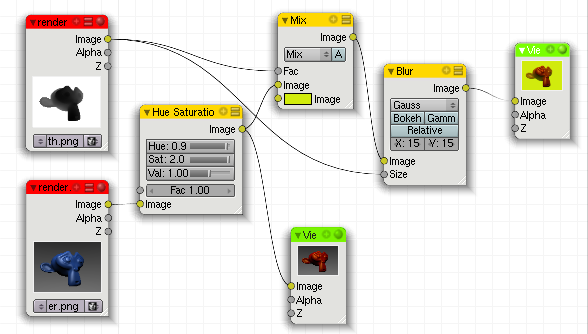
\includegraphics[width=0.6\textwidth]{images/nodes} }
				\subfloat[Image calculée par le graphe (a)]{ \label{fig:render-hsv} 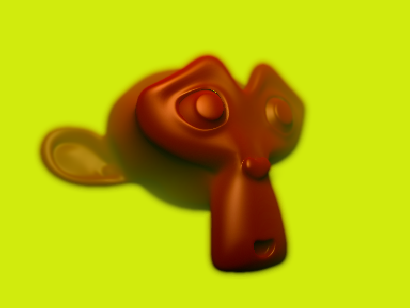
\includegraphics[width=0.4\textwidth]{images/nodes-out} }
				\caption{Example d'édition nodale d'images tel qu'implémenté par \emph{Blender 2.49}}
				\label{fig:editnodal}
			\end{figure}
			Les frameworks nodaux représentent l'image par un graphe composé de trois types de noeuds.
			\begin{itemize}
				\item Les noeuds d'entrée servent à spécifier les images à modifier et ne proposent que des sorties.
				\item Les noeuds d'opération prennent en entrée des images et/ou des canaux et/ou des paramètres,
				et proposent en sortie le résultat des images et/ou des canaux et/ou des valeurs, résultats de
				l'opération sur les entrées.
				\item Les noeuds de visualisation n'ont qu'une entrée et servent à visualiser sa valeur, que ce soit un paramètre,
				un canal ou une image. Dans le cas de canaux ou d'images, le noeud peut également spécifier une sous région
				de l'image et une échelle.
			\end{itemize}
			Le graphe est acyclique et dirigé; chaque arrète va de la sortie d'un noeud à une entrée d'un autre. Il peut
			y avoir plusieurs arrètes partant d'une sortie, mais une seule arrivant à chaque entrée. 
		
		\subsection{Algorithme de rasterisation}
			Pour obtenir la sortie d'un noeud, il faut premièrement obtenir toutes ses entrées, et appliquer l'opération du
			noeud s'il y en a une. On appliquera donc ce principe de manière récursive en partant d'un noeud de visualisation,
			la récursion s'arrètant au noeuds d'entrée.

			Si le noeud de visualisation spécifie une sous-région de l'image, l'algorithme fonctionne de manière identique, à
			ceci près que les opérations pouvant transformer géométriquement l'image, la région en entrée ne sera pas la même que
			la sortie. Il faut donc que le noeud soit capable d'inverser la transformation qu'il effectue afin de demander la bonne
			région à ses parents. 

			Si le noeud de visualisation spécifie une échelle, les images fournies par les noeuds d'entrée sont mises à l'échelle avant
			leur sortie, de même que les paramètres métriques des opérations. 

			Comme une sortie peut être connectée à plusieurs entrées, une même opération peut être calculée plusieurs fois. Pour éviter
			cela, chaque noeud peut disposer d'une cache dans laquelle il place le résultat de ses sorties. 

			Les images utilisées peuvent également utiliser une représentation par tiles afin de bénéficier des avantages de gestion d'images
			volumineuses.

		\subsection{Fonctionalités adaptées aux frameworks nodaux}
			\subsubsection{Édition non destructive}
				C'est un des gros points forts des frameworks nodaux. On peut facilement modifier les paramètres et la topologie du graphe
				et visualiser le résultat.
			\subsubsection{Modèle colorimétrique}
				Un framework nodal offre une liberté totale à l'utilisateur en ce qui concerne les modèles colorimétriques. Si un noeud sort
				une image en RGB, et qu'une opération attend du YUV, il peut les connecter ensemble. Le canal R sera interprété comme Y, le G comme
				U et le B comme V. S'il désire garder l'interprétation colorimétrique du RGB, il devra utiliser un noeud qui convertit le RGB en YUV.

				Intégrer un nouveau modèle colorimétrique se limite donc à créer des noeuds de conversions et les noeuds d'opération qui peuvent
				tirer bénéfice de ce nouveau modèle.
				
			\subsubsection{Images gigapixel}
				La complexité en temps et en mémoire de la rasterisation d'une image ne dépend tout au long du graphe que de la taille de
				la région du noeud de visualisation. Une borne supérieure de la taille de ces région est la résolution des écrans qui ne
				dépasse pas les quelques mégapixels. Il reste l'opération d'échelle à effectuer au niveau des région d'entrée. Si on
				dispose de mipmaps de ces images, alors il est possible d'effectuer des opérations sur images gigapixels de manière efficace.
			\subsubsection{Traitement d'images multiples}
				Le même graphe peut très facilement s'appliquer sur un grand nombre d'images de manière automatique.
				
		\subsection{Fonctionalités inadaptées aux frameworks nodaux}
			\subsubsection{Undo/Redo}
				On peut s'attendre d'un framework permettant l'édition non destructive d'exceller dans l'undo/redo. Cependant, il n'est pas
				facile de gérer les changements de paramètres des noeuds et de la topologie du graphe tout en maintenant des caches cohérentes.
				C'est pourquoi les graphes nécessitent souvent d'être rasterisés à nouveau ce qui peut prendre du temps lorsque celui ci contient
				des filtres complexes. 
			\subsubsection{Opération de dessin de primitves}
				Un dessin requiert plusieurs centaines de milliers d'opérations de dessin de primitives pour sa réalisation. Or un noeud d'un
				framework nodal est une entité complexe à gérer, et il devient impossible à l'utilisateur de gérer un graphe contenant autant
				de noeuds. Sans parler de la consommation en mémoire du graphe, et de le surcharge de calcul qu'entraine les connections de noeud.

				On ne peut pas non plus se permettre de devoir recalculer toutes les opérations de dessin à chaque Undo/Redo.

				Les frameworks nodaux font donc souvent le choix d'ignorer totalement les opérations de dessin. Celles-ci sont alors effectuées
				sur les images avant leur entrée dans le graphe, et doivent être gérées par un autre framework tel qu'un framework vectoriel ou bitmap.

				Certains frameworks nodaux choisissent de proposer des noeuds qui regroupent une séquence d'opération de dessin en une seule.
				Ces noeuds sont donc obligés de gérer par des mécanismes interne l'undo/redo. De tels noeuds fonctionnant comme des frameworks bitmaps
				ils ne peuvent pas gérer des opérations de dessin de trop grande taille.

	\section{Framework vectoriel}
		\subsection{Schéma de représentation de l'image}
			\begin{figure}[h]
				\centering
				\subfloat[l'image]{ \label{fig:render} 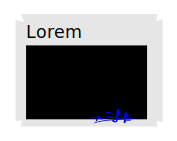
\includegraphics[width=0.33\textwidth]{images/scenegraph-img} }
				\subfloat[Le graphe de scène]{ \label{fig:render-hsv} 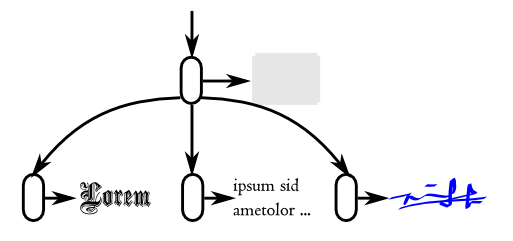
\includegraphics[width=0.66\textwidth]{images/scenegraph-graph} }
				\caption{Représentation d'une image par graphe de scène}
				\label{fig:editnodal}
			\end{figure}
			L'image est décrite par un emsemble de primitives géométriques. Ces primitives sont organisées dans un graphe de scène. Dans un 
			graphe de scène, chaque noeud représente une transformation géométrique et une primitive. La transformation géométrique détermine
			la position, l'échelle, et la rotation de la primitive et de ses enfants. La primitive est elle décrite par son type et les paramètres
			qui déterminent sa forme et son apparence.

			Le graphe de scène est acyclique. chaque noeud peut avoir plusieurs enfants et la plupart du temps un seul parent. 

			L'ordre des enfants d'un noeud est important puisqu'ils déterminent l'ordre dans lequel ils seront dessinés. Ainsi les derniers
			enfants d'un noeuds seront dessinés au dessus des premiers. 

			Chaque framework a sa propre liste de primitives géométriques, mais tous disposent au moins des points, lignes, ploygones, ellipses,
			texte, et courbes de bézier.

		\subsection{Algorithme de rasterisation}
			L'utilisateur commence d'abord par choisir la région qu'il veut rasteriser et à quelle résolution. Le framework crée ensuite un bitmap
			de cette taille et résolution de la couleur de fond de l'image.

			Pour dessiner un noeud du graphe, on applique sa transformation aux paramètres de sa primitive. On dessine ensuite cette 
			primitive sur le bitmap. On Dessine ensuite chaque noeud enfant dans l'ordre en leur appliquant la transformation de ce noeud.

			Cette opération est effectuée de manière récursive en partant du noeud racine de l'image.

			Afin d'éviter de dessiner les primitives qui se trouvent en dehors de la région à rasteriser, on associe à chaque noeud une boite
			qui englobe sa primitive ainsi que celles de tous ses enfants. Si la boite est en dehors de la région, on peut ignorer ce noeud et
			leurs enfants. 

			Afin d'exploiter l'accélération matérielle, la plupart des frameworks ne dessinent pas directement les primitives, mais les 
			convertissent en triangles qui sont ensuite dessinés à l'aide du matériel. Cette approche peut également s'avérer bénéfique 
			sans accélération matérielle car le dessin de triangle est souvent beaucoup plus rapide qu'un dessin analytique de la primitive,
			de plus les détails trop petits pour être vus peuvent être détectés lors de la transformation de la primitive en triangles.

		\subsection{Fonctionalités adaptées aux frameworks vectoriels}
			\subsubsection{Édition non destructive}
				La description de la scène étant gardée en mémoire, il est facile de la modifier et d'obtenir ensuite une nouvelle visualisation.
				L'algorithme de rasterisation ne disposant généralement pas de cache, l'intégralité de la région à visualiser doit être recalculée à chaque 
				modification de l'image. Cela n'est pas un problème tant que la taille du graphe de scène reste raisonnable.
			\subsubsection{Undo / Redo}
				L'undo/redo est simple à implémenter et aussi efficace que l'édition non destructive. 
			\subsubsection{Images gigapixel}
				Les frameworks vectoriels décrivant l'image de manière analytique peuvent gérer des images de toutes tailles et résolutions. De 
				plus la description vectorielle utilise beaucoup moins de mémoire. Ces frameworks sont pour l'instant la solution de 
				choix pour la description de telles images.
			\subsubsection{Opérations de dessin de primitives}
				Les frameworks vectoriels sont très pratiques pour éditer un dessin constitué de primitives géométriques. Cependant, la région de
				visualisation doit être rasterisée à chaque changement d'échelle ou à chaque déplacement de celle-ci. Si le nombre de primitives
				constituant le dessin est trop grand, ceci ne peut plus se faire de manière interactive.
				
				Les frameworks vectoriels sont donc généralement utilisés pour les documents textuels, les cartes, les graphes, ou les dessins abstraits
				qui peuvent être décrits par un petit nombre de primitives complexes. A contrario, les images peintes utilisent 
				un trop grand nombre de primitives pour que de tels frameworks soient efficaces.
		\subsection{Fonctionalités inadaptées aux frameworks vectoriels}
			\subsubsection{Filtres}
				En associant les filtres aux noeuds on s'attend à ce que le filtre ne s'applique
				qu'à ce noeud et à ses enfants. Ceci nécessite de faire une rasterisation de ces noeuds dans un buffer séparé afin d'y appliquer le
				filtre, puis de réintégrer ce buffer dans le buffer en cours. Et ce de manière récursive selon qu'il y ait des filtres dans les
				noeuds enfants. 
				Tout cela ralentit nettement la rasterisation, d'autant que le rendu dans de multiples buffer ne fait pas bon ménage avec 
				l'accélération matérielle. Les frameworks proposent parfois de tels filtres, mais les performances suivent rarement.
				
				D'autres frameworks proposent des filtres avec des sémantiques plus complexes. TODO

			\subsubsection{Modèles colorimétriques}
				Tant la description de l'image que l'algorithme de rasterisation sont peu adaptés au support de multiples modèles 
				colorimétriques, à une exception près, celui des systèmes halftone qui décrivent l'image non en couleurs RGB, mais en terme de 
				couches de couleurs correspondant aux encres disponibles à l'impression. 

	\section{Mégatexture ou VirtualTexture}
		Le Megatexturing est une technique plus qu'un framework à part entière. Le but de cette technique est de permettre l'affichage et l'édition
		d'images gigapixel en tant que textures de scènes 3D interactives.
		\subsection{Schéma de représentation de l'image}
			\begin{figure}[h]
				\centering
				\subfloat[La pyramide de tile représentant l'image complète]{ \label{fig:render} 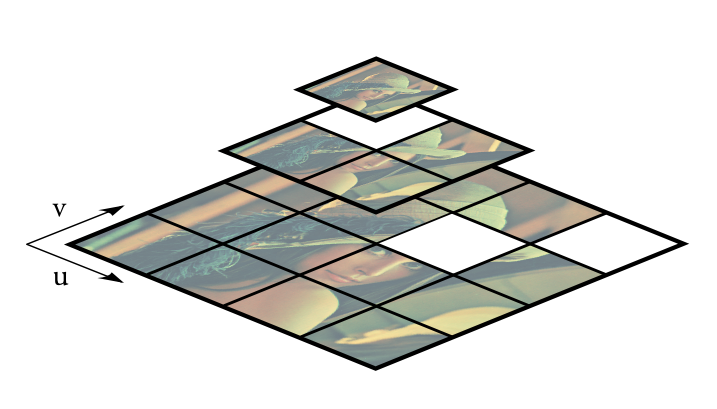
\includegraphics[width=0.6\textwidth]{images/megatextures-pyramid} }
				\subfloat[La texture virtuelle, composée de tiles de la pyramide]{ \label{fig:render-hsv} 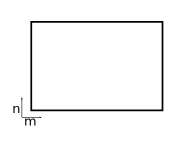
\includegraphics[width=0.4\textwidth]{images/megatextures-virtual} }
				\caption{Mégatexture}
				\label{fig:editmegatex}
			\end{figure}
		L'image est représentée par deux structures différentes, l'une se trouvant sur le disque et l'autre en mémoire.
		Celle qui se trouve sur le disque est la plus volumineuse des deux. Elle est composée d'une pyramide creuse de tiles. 

		Cette structure consiste en l'image gigapixel complète, divisée en tiles, les régions vides ou facultatives de l'image étant représentées par une absence
		de tiles, afin d'économiser de la mémoire. La structure contient aussi tous les mipmaps de cette image sous forme de tiles de dimensions identiques.

		En mémoire se trouve une texture, appellée \emph{texture virtuelle} qui a la taille maximum supportée par le matériel d'accélération, 
		ce qui est beaucoup moins que l'image originale. Cette texture est composée de tiles se trouvant dans la pyramide.
		
		\subsubsection{Affichage de l'image}
			Pour afficher une texture sur un maillage 3D, on assigne à chaque vertice  du maillage une coordonnée $u,v$ correspondant à un pixel de cette texture.
			de la texture. Comme nous désirons afficher la texture gigapixel, ces coordonnées correspondent aux pixels de cette texture.
			Cette texture est cependant trop grande pour pouvoir être utilisée telle quelle.
			
			Pour résoudre ce problème on place les tiles qui nous intéressent dans une texture virtuelle qui est suffisemment petite pour pouvoir
			être utilisée pour l'affichage. Un \emph{pixel shader} est ensuite utilisé pour traduire à l'affichage les coordonnées $u,v$ de la
			texture gigapixel en les coordonnées $m,n$ de la texture virtuelle. 

			Pour déterminer quels tiles nous intéressent, on s'aide d'un premier rendu dans lequel on examine quelles régions de la texture gigapixel
			sont affichées, et à quelle résolution. On sélectionne ensuite les tiles qui couvrent cette zone avec la résolution la plus proche de celle
			affichée. Comme la résolution de l'écran est plus petite que celle de la taille de la texture virtuelle, on disposera toujours d'une place
			suffisante pour couvrir la quantité de texture affichée.

		\subsubsection{Édition de l'image}
			Pour générer et éditer l'image gigapixel, on utilise la technique précédente pour l'affichage, et on utilise les techniques de framework 
			bitmap pour appliquer les opérations; Celles-ci sont directement rasterisées dans la pyramide de tiles.
	\section{Comparaison}
\chapter{Framework Himalaya (20 pages) }
	\section{Structures de données}
		\subsection{Frame}
		\subsection{Image}
		\subsection{Opérations}
		\subsection{États}
	\section{Algorithmes}
		\subsection{Rasterisation}
		\subsection{Dessin}
		\subsection{Sauvegarder l'état}
		\subsection{Charger un état}
		\subsection{Supprimer un état}
		\subsection{Modifier une opération}
	\section{Gestion de la cache}
	\section{Utilisation}
		\subsection{API publique}
		\subsection{Undo / Redo}
		\subsection{Modèle objet par calques}
		\subsection{Modèle objet nodal}
		\subsection{Traits de pinceau}

\chapter{Localité des operations (20 pages)}
	\section{Opérations vectorisées}
		\subsection{Impact sur l'API}
		\subsection{Évaluation des performances}
	\section{Bounding Boxes}
		\subsection{Algorithme Inline}
		\subsection{Algorithme Off-line}
		\subsection{Multi-Niveaux}
		\subsection{Impact sur l'API}
		\subsection{Évaluation des performances}

\chapter{Anti-aliasing (15 pages) }
	\section{Primitive de dessin}
	\section{Problèmes d'échelle}
		\subsection{Oversampling}
	\section{Problèmes de superposition}
	\section{Problèmes de bandes}
	\section{Problème de blending à faible opacité}
	\section{Problème de précision de positionement}
\chapter{Test utilisateurs (10 pages) }
	\section{Procédure}
	\section{Résultats}
	\section{Analyse}
\chapter{Comparaison d'Himalaya aux autres frameworks}
\chapter{Conclusion}
